\documentclass{article}
\usepackage[utf8]{inputenc}

\title{MATH 20C Notes - Week One}
\author{C-Rin}
\date{October 2019}

\usepackage{amssymb}
\usepackage{natbib}
\usepackage{graphicx}
\usepackage{gensymb}
\usepackage{amsmath}

\graphicspath{ {./images/} }

\begin{document}

\maketitle

\section*{Introduction}
This will be the beginning document for my collection of MATH 20C notes this quarter. 

\begin{figure}[h!]
\centering

\includegraphics[scale=0.09]{fish.png}
\caption{A Fish}
\label{fig:universe}
\end{figure}


\section{9/27/29 Lecture}
\subsection{Vectors in 2D and 3D}

Vectors are a quantity with both direction and magnitude that is shown in a tuple of numbers.

    \[(1,2)\]
    \[(4,5,6)\]
\subsection{Adding Vectors}
We are able to add vectors coordinate-wise, adding x-values together, y-values, and so on.


    \[\vec{v} = (a,b,c)\]
    \[\vec{w} = (d,e,f)\]
    \[\vec{v}+\vec{w} = (a+d,b+e,c+f)\]
\subsection{Real Number Notation}
For real numbers, $\mathbb{R}$ is used to notate real numbers and vectors, where
\[\mathbb{R} \mbox{ and } \mathbb{R}^1\mbox{ notate the set of real numbers}\]
\[\mathbb{R}^2\mbox{ notates the set of pairs of real numbers (2D Vectors)}\]
\[\mathbb{R}^3\mbox{ notates the set of 3D Vectors}\]

\subsection{Scaling Vectors}
We can also scale vectors using a real number $\lambda$, where
\[\lambda \mbox{ is a real number, }\mathbb{R}\]
\[\vec{w} = (a,b)\]
\[\lambda\vec{w}=(\lambda a,\lambda b)\]

\section*{Example}
Solve the equation $(-21,23)-(x,6)=(-25,y)$ for $x$ and $y$
\[\mbox{For } x,\]
\[-21-x=-25\mbox{;  } x=4\]
\[\mbox{For } y,\]
\[23-6=y\mbox{;  } y=17\]
\[x=4,y=17\]

\section{The Dot Product}
\subsection{Unit Vectors}
Also known as "Standard Basis Vectors," unit vectors 
describe the linear combination of vectors.
\[i=(1,0,0)\]
\[j=(0,1,0)\]
\[k=(0,0,1)\]
\[\vec{v}=(a,b,c)=a\hat{i}+b\hat{j}+c\hat{k}\]

$\vec{v}$ is a linear combination of $\hat{i},\hat{j},\hat{k}$

\subsection{The Inner/Dot Product}
There are a few ways to multiply vectors, of which we have 
already discussed scalar multiplication, where we multiply 
a vector with a real number. Another method we can use is the 
\textbf{Dot Product}, also known as the inner product.

\subsection*{Example}
The Dot Product of $\vec{v}=(a,b,c)$ and $\vec{w}=(d,e,f)$ is the real number

\[ \vec{v}\cdot \vec{w}=a\cdot d +b\cdot e+ c\cdot f\]

We can multiply each corresponding coordinate and add them together.

\subsection{The Length of a Vector}
The length of a vector can be found with 
\[ \vec{v}=\sqrt{a^2 +b^2 +c^2}=\sqrt{\vec{v}\cdot \vec{v}}\]

A unit vector is a vector of length, and any non-zero vector $\vec{v}$ is 
a scalar multiple of a unit vector.
\newline
A 2D vector with a length of 1 creates a unit circle with a radius of 1, while 
a 3D vector with a length of 1 creates a sphere with radius 1.

\[ \vec{v}=||\vec{v}||\overbrace{(\frac{\vec{v}}{||\vec{v}||})}^{\mbox{unit vector}}\]

\subsection{The Geometric Interpretation of the Dot Product}
Let $\vec{v}$ be a non-zero vector with a normalized vector $\vec{u}$

\[ \vec{u}\cdot \vec{v}=\overbrace{||\vec{v}||}^{\mbox{length of $\vec{v}$}}\]

\[ \vec{v}=||\vec{v}||\cdot \vec{u}\]
\[ \vec{u}\cdot \vec{v}=\vec{u}\cdot \]

If $\vec{v}$ and $\vec{w}$ point in the same direction, then $\vec{v}\cdot 
\vec{w}=||\vec{v}||\cdot ||\vec{w}||$

\section{The Law of Cosines}
\[||\vec{u}-\vec{v}||^2 = ||\vec{u}||^2 + ||\vec{v}||^2 +2||\vec{u}||\cdot||\vec{v}||\cos(\theta) \]

\[ 2\cos(\theta)=\vec{u}\cdot\vec{u}+\vec{v}\cdot \vec{v}-(\vec{u}-\vec{v})(\vec{u}-\vec{v})=2\vec{u}\cdot \vec{v} \]

\subsection{Master Equation}
For any two vectors $\vec{v},\vec{w}$
\[\vec{v}\cdot \vec{w}=||\vec{v}||\cdot ||\vec{w}||\cos(\theta)\]

The two vectors $\vec{v},\vec{w}$ are perpendicular if and only if  $\vec{v}\cdot \vec{w}=0$

\subsection*{Example}
What is the angle between $2\hat{j}-\hat{i}$ and $\hat{i}+\hat{j}$

\[(\hat{i}+\hat{j})\cdot(2\hat{j}-\hat{i})=||\hat{i}+\hat{j}||\cdot ||2\hat{j}-\hat{i}||\cos(\theta) \]
\[(\hat{i}+\hat{j})\cdot(2\hat{j}-\hat{i})=-1+2=1 \]
\[||\hat{i}+\hat{j}||=\sqrt{1^2 +1^2}=\sqrt{2}\]

\subsubsection{Compute the angle between $\hat{i}=(1,0)$ and $\hat{j}=(0,1)$}
\[\theta=90\degree\]
\subsubsection{Compute the angle between $(2,4)$ and $(3,7)$}
\[(2,4)\cdot(3,7)=\sqrt{20}\cdot\sqrt{58}\cos(\theta)\]
\[(6+28)=\sqrt{20}\cdot\sqrt{58}\cos(\theta)\]
\[\cos(\theta)=\frac{34}{\sqrt{20\cdot 58}}\]
\[\theta=\arccos(\frac{\vec{v}\cdot\vec{w}}{||\vec{v}||\cdot ||\vec{w}||})\]

\subsection{Cauchy-Schwarz Inequality}
\[|\vec{v}\cdot \vec{w}|\leq ||\vec{v}||\cdot||\vec{w}||\]
\[\vec{a}\cdot \vec{v}=||\vec{a}||\cdot ||\vec{b}||\cos(\theta)\]

The equality hold exactly when $\vec{v}$ and $\vec{w}$ are scalar multiples of each other

\section{Orthogonal Projection}
Vectors are orthogonal when they are perpendicular, so the dot product of two vectors that are 
perpendicular equal zero.
\[\vec{p} \mbox{ is a vector on the line through }\vec{o}\mbox{ (the origin)}\mbox{ in the direction of }\vec{w}\]
\[\vec{q} \mbox{ is perpendicular (orthogonal) to }\vec{w}\]
\[\mbox{So }\vec{q}\cdot\vec{w}=0\]

\subsection{Definition}
\[\vec{p} \mbox{ is the projection of } \vec{v} \mbox{ onto }\vec{w}\]
How do we find $\vec{p}$
\[\vec{p}=\lambda\vec{w}\mbox{ for some real number }\lambda\]
\[\vec{q}=\vec{v}-\vec{p}=\vec{v}-\lambda\vec{w}\]
\[0=\vec{w}\cdot\vec{q}=\vec{w}\cdot\vec{v}-\lambda\vec{w}\cdot \vec{w}\]
\newline
Solve for $\lambda$
\[\vec{w}\cdot \vec{v}=\lambda(\vec{w}\cdot\vec{w})\]
\[\mbox{For }\lambda=\frac{\vec{w}\cdot\vec{v}}{\vec{w}\cdot\vec{w}}\]
\[\vec{p}=\frac{\vec{w}\cdot\vec{v}}{\vec{w}\cdot\vec{w}}\cdot \vec{w}\]

\subsection*{Example}
\[\vec{v}=(2,2) \mbox{;}\vec{w}=(1,2)\]
We want to find the orthogonal projection of $\vec{v}$ onto $\vec{w}$

\[\vec{p}=\frac{\vec{w}\cdot\vec{v}}{\vec{w}\cdot\vec{w}}\cdot \vec{w}=\frac{(1,2)\cdot (2,2)}{(1,2)\cdot(1,2)}\cdot(1,2)\]
\[=(\frac{6}{5})(1,2)=(\frac{6}{5},\frac{12}{5})\]

\subsection*{Exercise}
Find the orthogonal projection of (1,2,3) onto (1,1,1)
\[\vec{p}=\frac{(1,1,1)\cdot(1,2,3)}{(1,1,1)\cdot(1,1,1)}(1,1,1)\]
\[=\frac{1+2+3}{1+1+1}(1,1,1)=\frac{6}{3}(1,1,1)=2(1,1,1)=(2,2,2)\]

\section{The Triangle Inequality}
\begin{figure}[h!]
    \centering
    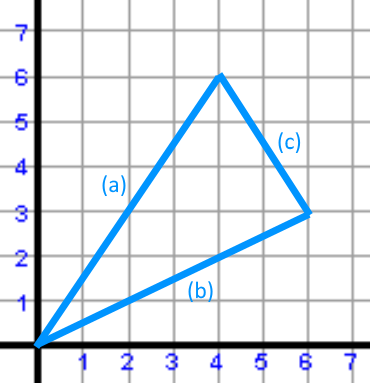
\includegraphics[scale=.5]{TriangleInequality.png}
    \label{}
\end{figure}
For any two vectors $\vec{a}$ and $\vec{b}$
\[\overbrace{||\vec{a}-\vec{b}||}^{\mbox{Distance between $\vec{a}$ and $\vec{b}$}}\leq\overbrace{||\vec{a}||}^{length of \vec{a}}+||\vec{b}||\]
In 2D, the length of the third edge of a triangle is at most the sum of the lengths of the other sides.

\[||b-a|| \leq ||a||+||b||\]
\[||a+b|| \leq ||a||+||b||\]


\section{Matrices, Determinants, and the Cross Products}
A 2x2 matrix is an array of vectors

\[\overbrace{(a,b)}^{vector}\]
\[\overbrace{\begin{bmatrix}
    a&b\\
    c&d
\end{bmatrix}}^{matrix}\]
Each vector inside the matrix is a row vector

\subsection{Determinants}
The \textbf{determinant} of a 2x2 matrix is 
\[\begin{bmatrix}
    a&b\\
    c&d
\end{bmatrix}=ad-bc\]

\subsection*{Example}

\[\begin{bmatrix}
    1&1\\
    1&1
\end{bmatrix}=1\cdot 1-1\cdot 1=0\]

\[\begin{bmatrix}
    1&2\\
    3&4
\end{bmatrix}=1\cdot 4-2\cdot 3=4-6=-2\]

\subsection{Geometric Meaning}
The absolute value of the determinant equals to the area of the parallelogram of the matrix.
\begin{figure}[h!]
    \centering
    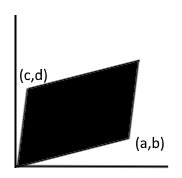
\includegraphics[scale=1.0]{geomeandeterminant.png}
    \label{}
\end{figure}
\begin{figure}[h!]
    \centering
    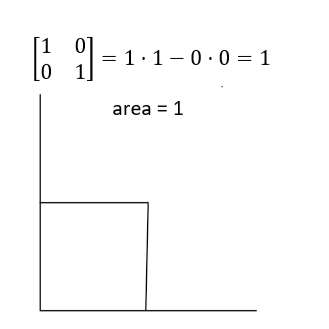
\includegraphics[scale=0.5]{2D-DeterminantExample.png}
    \label{}
\end{figure}

\[\begin{bmatrix}
    a&b\\
    c&d
\end{bmatrix}=0 \mbox{ exactly when$(a,b)$ and $(c,d)$ lie on the same line through $(0,0)$}\]

\section{3x3 Determinants}
When we move from 2D determinants to 3D, some changes must be made
\begin{itemize}
    
    \item In 2D, we make a parallelogram
    \begin{itemize}
        \item The absolute value of the 2D determinant equals to the area
    \end{itemize}
    \item In 3D, we make a parallelepiped
    \begin{itemize}
        \item The absolute value of the 3D determinant equals to the volume
    \end{itemize}
    \item Row vectors still make sense in 3D
\end{itemize}

\[\begin{bmatrix}
    \boldsymbol{a}&\boldsymbol{b}&\boldsymbol{c}\\
    d&e&f\\
    g&h&i
\end{bmatrix}=a\cdot\begin{bmatrix}
    e&f\\h&i
\end{bmatrix}-b\cdot\begin{bmatrix}
    d&f\\
    g&i
\end{bmatrix}+c\begin{bmatrix}
    d&e\\
    g&h
\end{bmatrix}\]


\begin{figure}[h!]
    \centering
    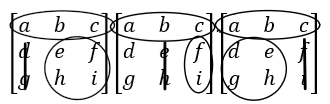
\includegraphics[scale=1]{derive3D-DeterminantForm.png}
    \label{}
\end{figure}

\begin{figure}[h!]
    \centering
    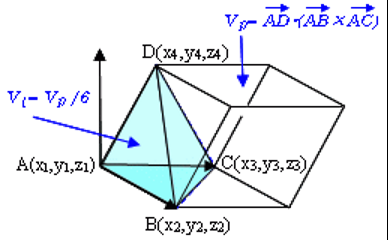
\includegraphics[scale=1]{parallelepiped.png}
    \caption{The shape created by the 3D determinant is a parallelepiped}
    \label{}
\end{figure}

\end{document}
